\documentclass[tikz,border=3mm]{standalone}
\usepackage[T1]{fontenc}
\usetikzlibrary{arrows.meta,positioning}
\begin{document}
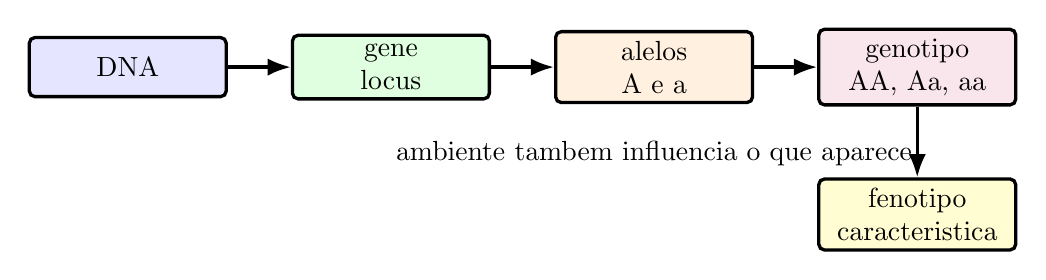
\begin{tikzpicture}[>=Latex,node distance=0.8cm]
  \tikzstyle{box}=[draw,rounded corners=2pt,very thick,align=center,minimum width=2.5cm,minimum height=0.75cm]
  \node[box,fill=blue!10] (dna) {DNA};
  \node[box,fill=green!12,right=0.8cm of dna] (gene) {gene\\locus};
  \node[box,fill=orange!12,right=0.8cm of gene] (alelo) {alelos\\A e a};
  \node[box,fill=purple!10,right=0.8cm of alelo] (geno) {genotipo\\AA, Aa, aa};
  \node[box,fill=yellow!18,below=0.9cm of geno] (fen) {fenotipo\\caracteristica};
  \draw[very thick,->] (dna) -- (gene);
  \draw[very thick,->] (gene) -- (alelo);
  \draw[very thick,->] (alelo) -- (geno);
  \draw[very thick,->] (geno) -- (fen);
  \node[align=center,below=0.35cm of alelo] {ambiente tambem influencia o que aparece};
\end{tikzpicture}
\end{document}
